\documentclass[12pt]{scrartcl}
\usepackage[sexy]{evan}
\usepackage{graphicx}

 %Sets
\newcommand{\N}{\mathbb{N}}
\newcommand{\Z}{\mathbb{Z}}
\newcommand{\F}{\mathbb{F}}
\newcommand{\Q}{\mathbb{Q}}
\newcommand{\R}{\mathbb{R}}
\newcommand{\C}{\mathbb C}
\newcommand{\T}{\mathbb T}

\let \phi \varphi
\let \hat \widehat

\newcommand{\<}{\langle}
\renewcommand{\>}{\rangle}


%From Topology
\newcommand{\cT}{\mathcal{T}}
\newcommand{\cB}{\mathcal{B}}
\newcommand{\cC}{\mathcal{C}}
\newcommand{\cH}{\mathcal{H}}
\renewcommand{\arc}{\text{arc}}


\usepackage{answers}
\Newassociation{hint}{hintitem}{all-hints}
\renewcommand{\solutionextension}{out}
\renewenvironment{hintitem}[1]{\item[\bfseries #1.]}{}
\declaretheorem[style=thmbluebox,name={Theorem}]{thm}
\declaretheorem[style=thmbluebox,name={Problem}]{Prob}


\begin{document}
\title{Olympiad Geometry}
\author{Vishal Raman}
\maketitle
\begin{abstract}
I first present my notes from the Art of Problem Solving(AoPS) Olympiad Geometry courses.  This includes problems, solutions and expository material.
\end{abstract}
\tableofcontents
\pagebreak
\section{Week 1: Fundamentals of Geometry}
\subsection{Similar Triangles}
The first fundamental tool at our disposal is similar triangles, which give us relationships between the lengths and angles of segments.  \begin{definition} Two triangles $\triangle ABC, \triangle DEF$ and similar (denoted $\triangle ABC \sim \triangle DEF$) if $\angle A = \angle D$, $\angle B = \angle E$, and $\angle C = \angle F$.  If the above relations hold, then we also have
$$\frac{AB}{DE} = \frac{BC}{EF} = \frac{CA}{FD}.$$
\end{definition}

Similar triangles can be useful if a problem involves ratios or products of lengths.  Another use(though rare) is that we show triangles are similar by showing $AB/DE = AC/DF = BC/EF$ and deduce the angles are equal.  We could also show that pair of sides have equal ratio and the included angle is equal: $AB/DE = AC/DF$ and $\angle BAC = \angle EDF$, then $\triangle ABC \sim \triangle DEF$.

We begin by present some applications.
\begin{thm}[Angle Bisector] Take $\triangle ABC$.  If $D \in BC$ so that $AD$ bisects $\angle BAC$, then $AB/BD = AC/CD$.
\end{thm}
\begin{proof}
Draw a line through $C$ parallel to $AB$ and mark $E$ as the insertion of the parallel line through $C$ and the extension of $AD$. 
\begin{center}
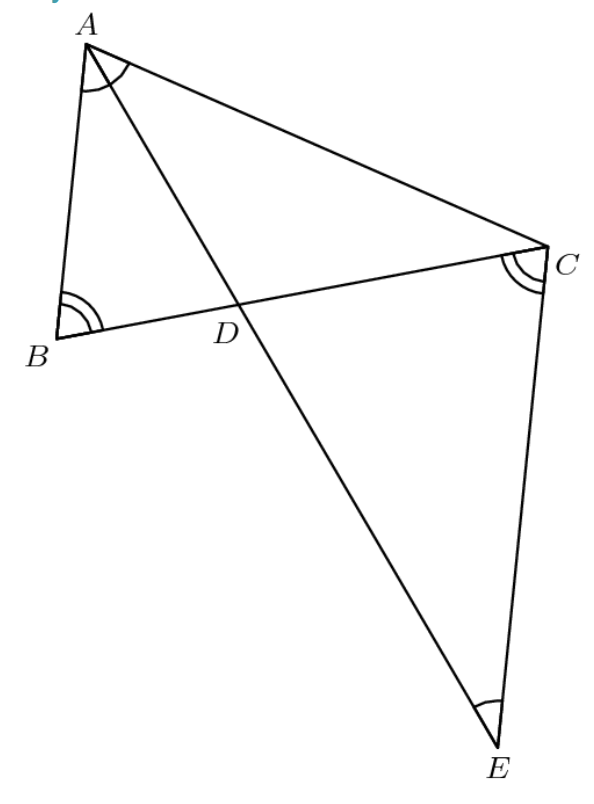
\includegraphics[scale=0.5]{graphics/angBis.png}
\end{center}

Then $\angle ABC = \angle ECD$ and $\angle DEC = \angle DAC$ so it follows that $\triangle ABC \sim \triangle ECD$.  Thus, $AB/BD = EC/CD$.  Finally, $\angle CED = \angle DAC$ so it follows that $\triangle ACE$ is isosceles and $AC = EC$ so we find that 
$$\frac{AB}{BD} = \frac{AC}{CD},$$
as desired.
\end{proof}
\begin{remark} We also could prove this using the Law of Sines or the ratio of areas of the two triangles.
\end{remark}

\begin{Prob} Given that $AB || CD || EF$, prove that $\frac{1}{AB} + \frac{1}{EF} = \frac{1}{CD}$ in the following diagram:
\begin{center}
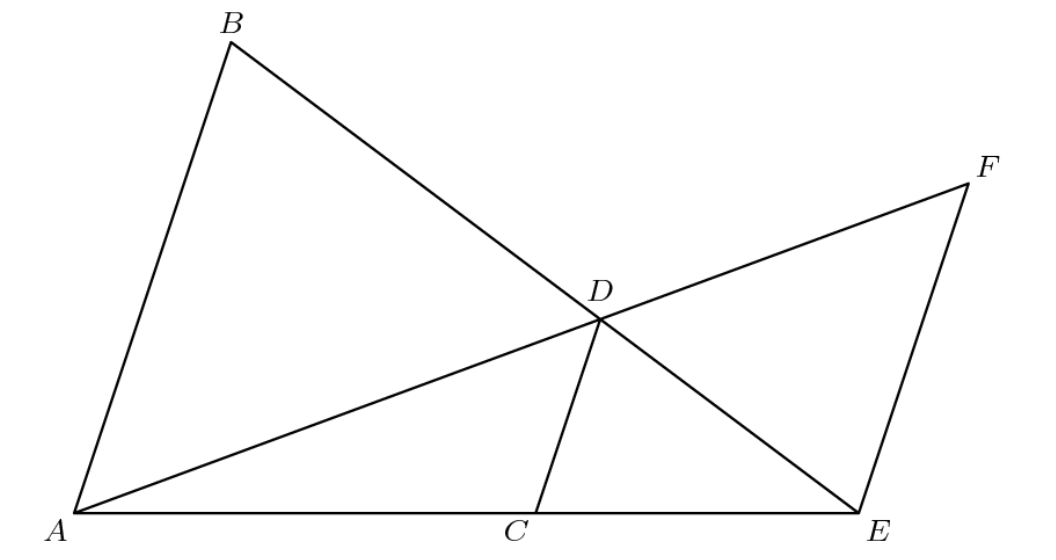
\includegraphics[scale=0.5]{graphics/simTri.png}
\end{center}
\end{Prob}
\begin{proof}
Multiplying through by $CD$, we get that 
$$CD/AB + CD/EF = 1.$$

Note that $\triangle ACD \sim \triangle AEF$ and $\triangle ECD \sim \triangle EAB$ so it follows that $CD/AB = CE/AE$ and $CD/EF = CA/AE$.

Finally,
$$\frac{CD}{AB} + \frac{CD}{EF} = \dfrac{CE}{AE}+\dfrac{CA}{AE} = \dfrac{AE}{AE} = 1.$$
\end{proof}

\subsection{Power of a Point}
\begin{thm}[Power of a Point] Take a point $P$ and circle $O$.  For any line that passes through $P$ and intersects $O$ at two points $X$ and $Y$, the product $(PX)(PY)$ is constant.  We call this product the \textbf{power of point} $P$ with respect to circle $O$.  
 \end{thm}
 \begin{center}
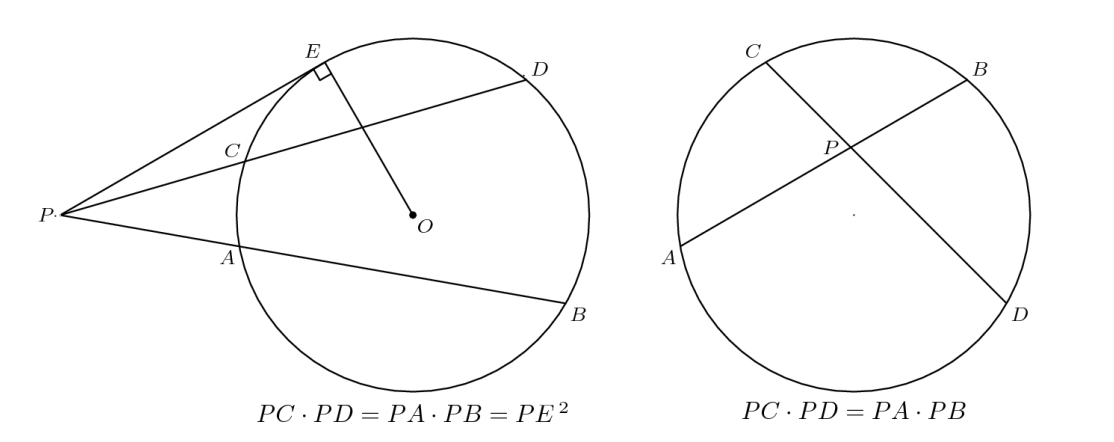
\includegraphics[scale=0.8]{graphics/pop.png}
\end{center}
The Power of a Point Theorem follows from similar triangles:
\begin{center}
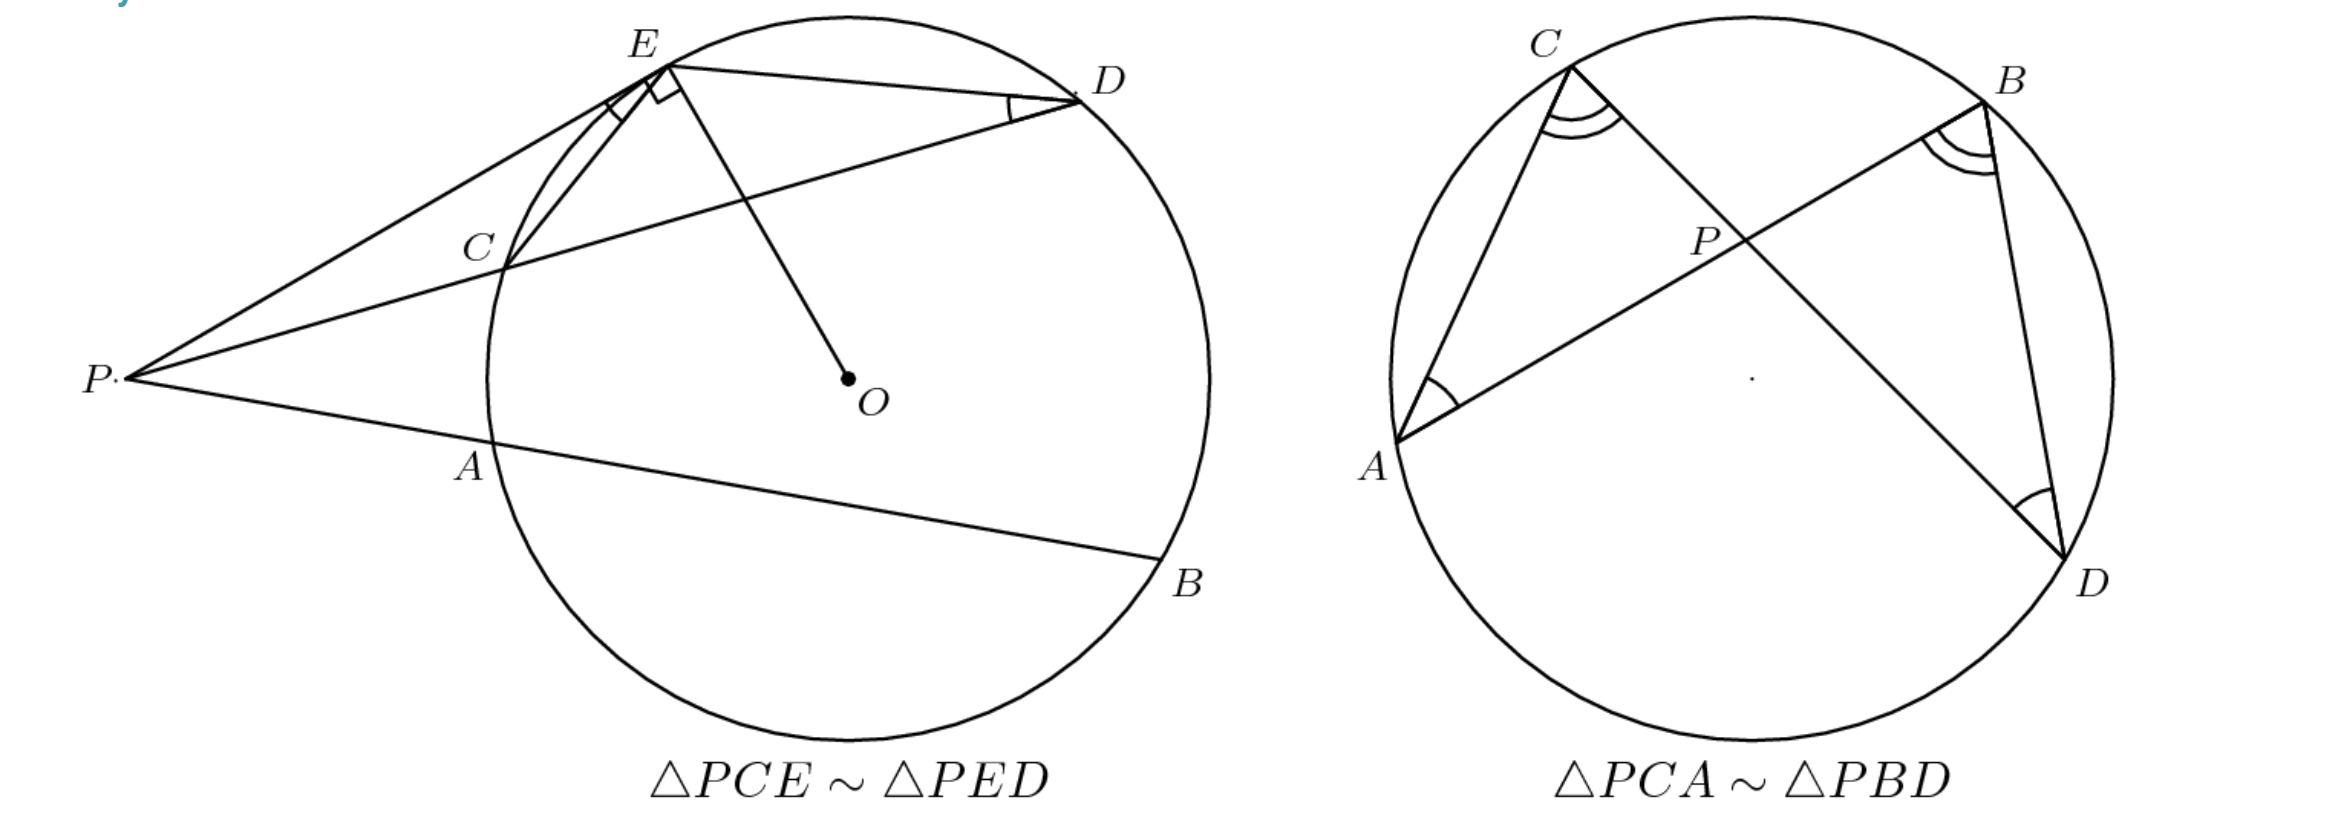
\includegraphics[scale=0.4]{graphics/popproof.png}
\end{center}
\begin{Prob} $AB$ is a diameter of circle $O$. Points $C$ and $D$ are on the circle such that $D$ bisects arc $AC$.  Point $E$ is on the extension of $BC$ that that $BE$ is perpendicular to $DE$.  $F$ is the intersection of $AE$ and circle $O$.  Prove that the extension of $BF$ bisects segment $DE$ at $M$. 
\end{Prob}
\begin{center}
\includegraphics[scale=0.6]{graphics/PoPp1.png}
\end{center}
\begin{proof}
We first claim that $OD || EB$.  This is because $$\angle AOD = \text{arc}(AD) = \text{arc}(AC)/2 = \angle ABE.$$
It follows that $ED$ is tangent to the circle, since $\angle ODE$ is a right angle.  Furthermore, $\angle AFB$ is a right angle since $AB$ is the diameter of the circle.  Now, note that $\text{Pow}_O(M) = MD^2 = MF \cdot FB.$  It suffices to show that $EF^2 = MF \cdot FB$.  This follows from the fact that $MFE \sim EFB$, so it follows that 
$$\dfrac{EF}{FB} = \dfrac{ME}{FE} \Longrightarrow EF^2 = ME \cdot FB.$$
\end{proof}
\subsection{Cyclic Quadrilaterals}
\begin{definition} A quadrilateral is called \textbf{cyclic} if a circle can be drawn that passes through all four vertices.
\end{definition}
There are 4 equivalent methods to showing a quadrilateral $ABCD$ is cyclic, namely:
\begin{itemize}
\item Showing $\angle ABD = \angle ACD$(or any of the other pairs of similarly defined angles).
\item Showing a pair of opposite angles sum to $180$ degrees.
\item The converse of the Power of a Point: if $P$ is the intersection of lines $AB$ and $CD$ and 
$$PA \cdot PB = PC \cdot PD$$
or 
$$QC \cdot QD = QB \cdot QA,$$
then $A, B, C, D$ are all on a circle.
\item The equality condition of \textbf{Ptolemy's Inequality}: In a quadrilateral $ABCD$, 
$$AB \cdot CD + BC \cdot DA \ge AC \cdot BC,$$
with equality if and only if $ABCD$ is cyclic.
\end{itemize}
I omit the basic examples but present some of the interesting ones:
\begin{proposition} A chord $ST$ of constant length slides around a semicircle with diameter $AB$.  $M$ is the midpoint of $ST$ and $P$ is the foot of the perpendicular from $S$ to $AB$.  Prove that the angle $SPM$ is constant for all positions of $ST$.
\end{proposition}
\begin{proof}
If $SM = MT$, then it follows $M$ is the perpendicular bisector of $\triangle OST$.  Thus, $OPSM$ is cyclic and $\angle SPM = \angle SOM$.  Finally, the length of $SM$ is constant, so it follows that the arc between intersection of the extension of $OM$ and the circle and $S$ is constant.  Thus, $\angle SPM$ is constant, as desired.
\end{proof}

\begin{proposition} $ABC$ is an acute triangle with $O$ as its circumcenter.  Let $S$ be the circle through $C, O, B$.  The lines $AB$ and $AC$ meet circle $S$ again at $P$ and $Q$, respectively.  Show that $AO$ and $PQ$ are perpendicular.  
\end{proposition}
\begin{center}
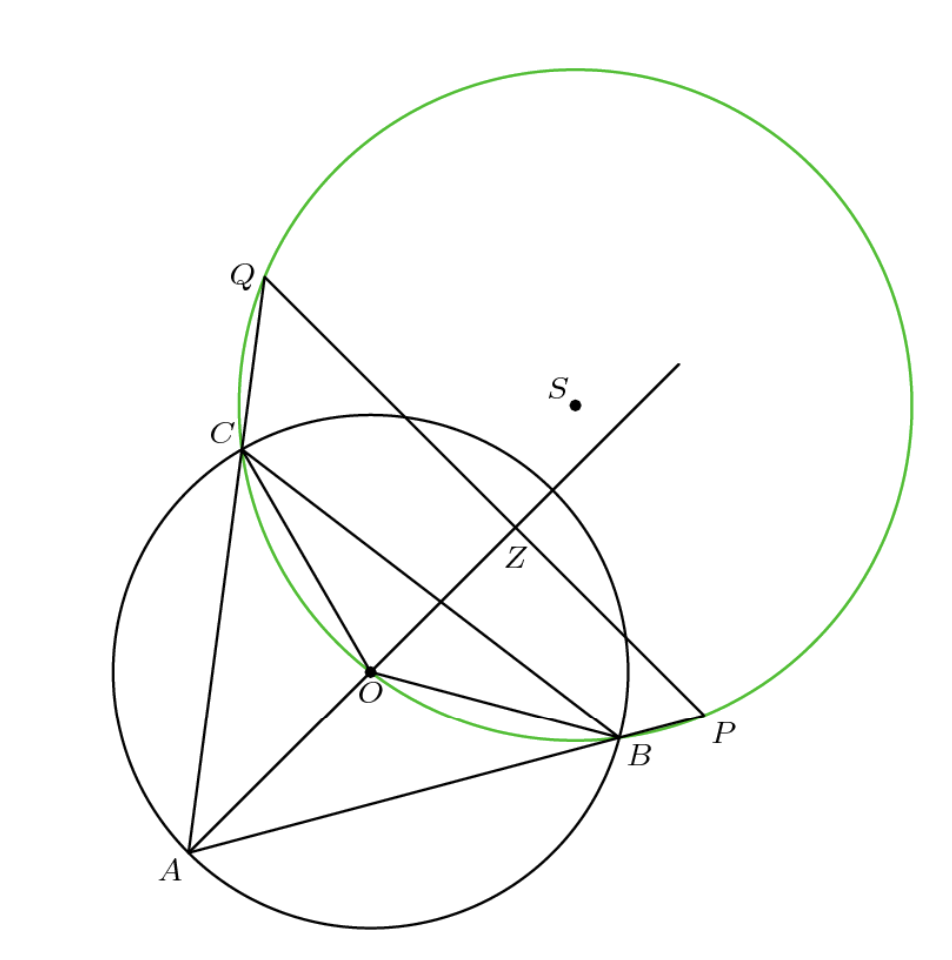
\includegraphics[scale=0.6]{graphics/CQp1.png}
\end{center}
\begin{proof}
It suffices to show that $\angle AZP$ is right, where $Z = AO \cap PQ$.  This reduces to showing that $\angle ZPA + \angle ZAP = 90$.  Since $PBCQ$ is cyclic, note that 
$$\angle ZPA = 180 - \angle BCQ = \angle ACB,$$
so it suffices to show that $ACB + OAB = 90$.  Mark $D$ as the intersection of $AO$ with the original circle.  Then, 
$$\angle ACB + \angle OAB = \frac{\text{arc}(AB) + \text{arc}(BD)}{2} = \frac{\text{arc}(AD)}{2} = 90.$$
\end{proof}
\subsection{Problems}
\begin{Prob} Let $ABC$ be a triangle and $D$ be the foot of the altitude from $A$. Let $E$ and $F$ be on a line passing through $D$ such that $AE$ is perpendicular to $BC$, $AF$ is perpendicular to $CF$, and $E$ and $F$ are different from $D$.  Let $M$ and $N$ be the midpoints of the line segments $BC$ and $EF$, respectively.  Prove that $AN$ is perpendicular to $NM$.
\end{Prob}
\begin{center}
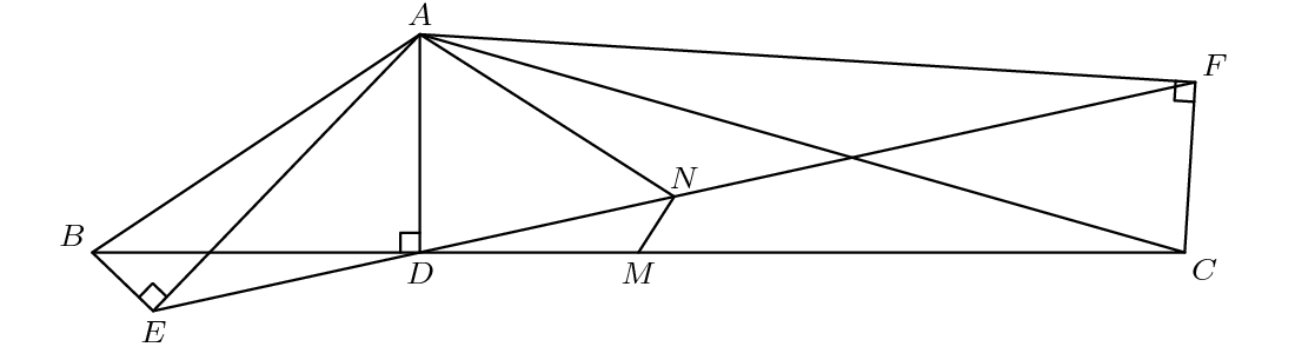
\includegraphics[scale=0.6]{graphics/p1-1.png}
\end{center}
\begin{proof}
Note that $ABED$ and $AFCD$ are cyclic quadrilaterals.  It follows that $ABC \sim AEF$ since $\angle ABD = \angle AED$ and $\angle AFD = \angle ACD$.  Similarly, we can show that $ABM \sim AEN$ since 
$$\frac{AB}{AE} = \frac{BC}{EF} = \frac{2BN}{2EM} = \frac{BN}{EM}.$$
Therefore, $\angle AND = \angle AMD$ and it follows that $ANMD$ is cyclic.  Therefore $\angle ANM = 180-\angle AD = 90$, as desired.
\end{proof}
\begin{Prob} Let $ABCD$ be a convex quadrilateral inscribed in a semicircle with diameter $AB$.  The lines $AC$ and $BD$ intersect at $E$ and the lines $AD$ and $BC$ meet at $F$.  The line $EF$ meets the semicircle at $G$ and $AB$ at $H$.  Prove that $E$ is the midpoint of $GH$ if and only if $G$ is the midpoint of the line segment $FH$.
\end{Prob}
\begin{center}
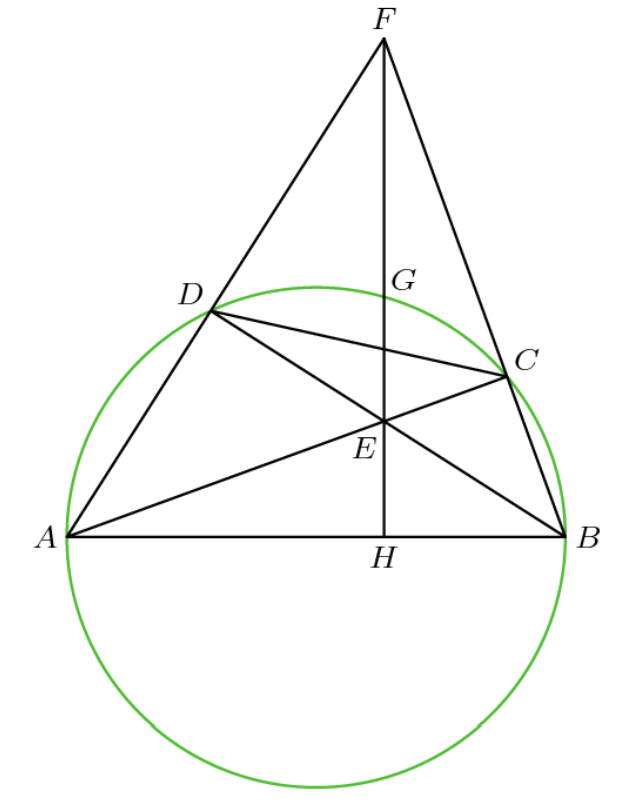
\includegraphics[scale=0.6]{graphics/p1-2.png}
\end{center}
\begin{proof}
Note that $\angle ADB = \angle ACB = 90$.  It follows that $E$ is the orthocenter of $FAB$ and $\angle FAH = 90$. We obtain many similar triangles, with one notable one begin $\triangle AEH = FBH$ which gives the relation 
$$HE \cdot HF = HA \cdot HB.$$
However, note that 
$$\text{Pow}(H) = HG^2 = HA \cdot HB,$$
so it follows that 
$$\frac{HG}{HF} = \frac{HE}{HG},$$
which proves the result.
\end{proof}
\pagebreak
\section{Homework 1: Fundamentals of Geometry}
\subsection{Problem 1}
\begin{Prob}
Let $ABCD$ be a quadrilateral such that all sides have equal length and $\angle ABC = 60$.  Let $k$ be a line through $D$ and not intersecting the quadrilateral.  Let $E$ and $F$ be the intersection of $k$ with lines $AB$ and $BC$ respectively.  Let $M$ be the point of intersection of $CE$ and $AF$.  Prove that $CA^2 = CM \cdot CE$. 
\end{Prob}
\begin{center}
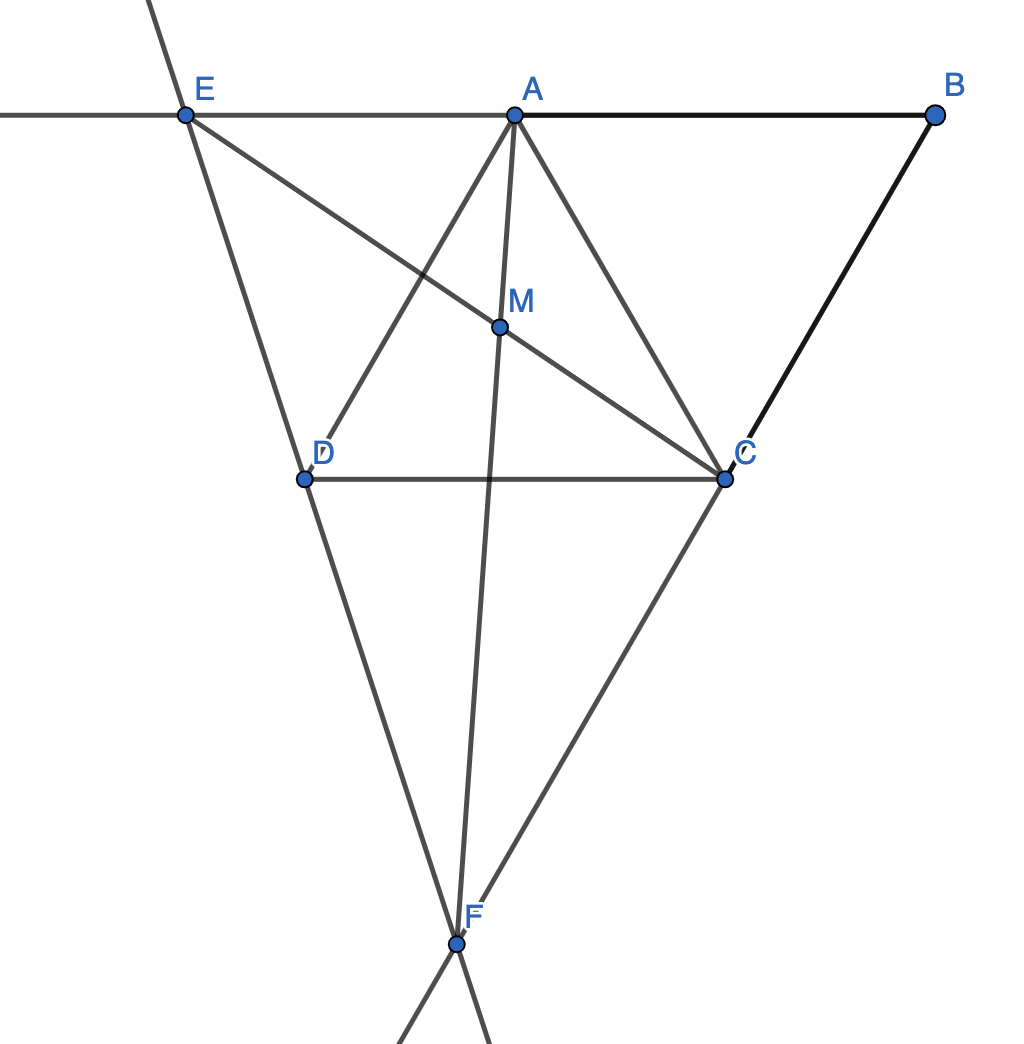
\includegraphics[scale=0.4]{graphics/hw1-1.png}
\end{center}
\begin{proof}
It suffices to show that $\triangle MCA \sim \triangle ACE$.  We already have that $\angle MCA = \angle ACE$ so we finish by showing that $\angle CAM = \angle CEA$.

We first claim that $AD || CB$ and $AB || DC$.  Note that $AB = BC$ and $\angle ABC = 60$ so it follows that $\triangle ABC$ is equilateral.  Hence $AB = CB = CA$.  But note that $AD = DC = AB = CA$, so it follows that $\triangle ADC$ is also equilateral.  Hence $\angle DAB = 120$ and $\angle ADC = \angle ABC = 60$ showing that $AD || CB$ and $AB || DC$.

Note that $\angle EAC = \angle ACE = 120$, so it suffices to show that $\frac{EA}{AC} = \frac{AC}{CF}$, since it follows that $\triangle EAC = \triangle ACF$ and $\angle CAM = \angle CEA$.  Furthermore, we have that $\triangle DCF \sim \triangle EAD$ since $\angle EAD = \angle DCA$ and $\angle AED = \angle CDF$.  It follows that 
$$\frac{EA}{AC} = \frac{DA}{FC} = \frac{AC}{FC},$$
since $DA = AC$, which completes the proof.
\end{proof}
\pagebreak
\subsection{Problem 2}
\begin{Prob} Let $C_1$ and $C_2$ be concentric circles with $C_2$ inside $C_1$.  Let $A$ and $C$ be on $C_1$ such that $AC$ is tangent to $C_2$ at $B$.  Let $D$ be the midpoint of $AB$.  A line passing through $A$ meets $C_2$ at $E$ and $F$ such that the perpendicular bisectors of $DE$ and $CF$ meet at a point $M$ on a segment $DC$.  Find the ratio $AM/MC$.
\end{Prob}
\begin{center}
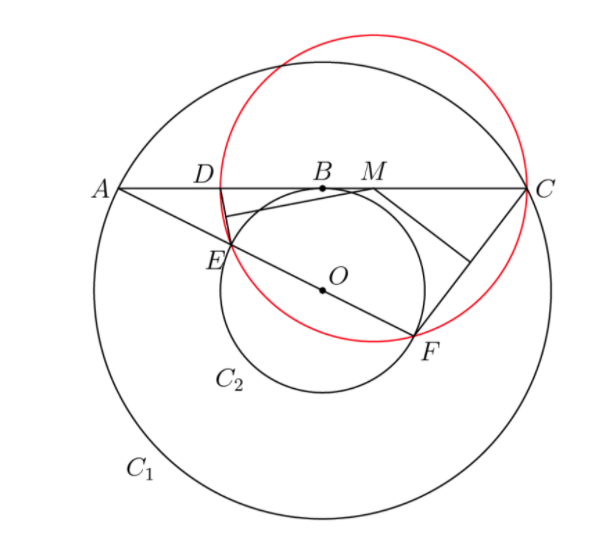
\includegraphics[scale=0.4]{graphics/hw1-2.png}
\end{center}
\begin{proof}
Note that $\text{Pow}_{C_2}(A) = AB^2 = AE \cdot AF$.  Furthermore, since $AD = \frac{1}{2}AB$ and $AC = 2AB$, it follows that 
$$AD \cdot AC = \frac{1}{2}AB \cdot 2AB = AB^2 = AE \cdot AF.$$
Hence, $DCFE$ is a cyclic quadrilateral.  Furthermore,  Since $M$ is the perpendicular bisector of the chords $DE$ and $CF$, it follows that $M$ is the center of the corresponding circle.  Hence $M$ is the midpoint of $DC$.  It follows that $AM = \frac{5}{8}AC$ and $MC = \frac{3}{8}AC$ so $AM/MC = 5/3$.
\end{proof}
\pagebreak
\section{Week 2: Fundamentals, Continued}
\subsection{Warm-up Problem}
\begin{Prob} $\triangle ABC$ is acute; $BD$ and $CE$ are altitudes.  Points $F$ and $G$ are the feet of perpendiculars $BF$ and $CG$ to line $DE$.  Prove that $EF = DG$.
\end{Prob}
\begin{center}
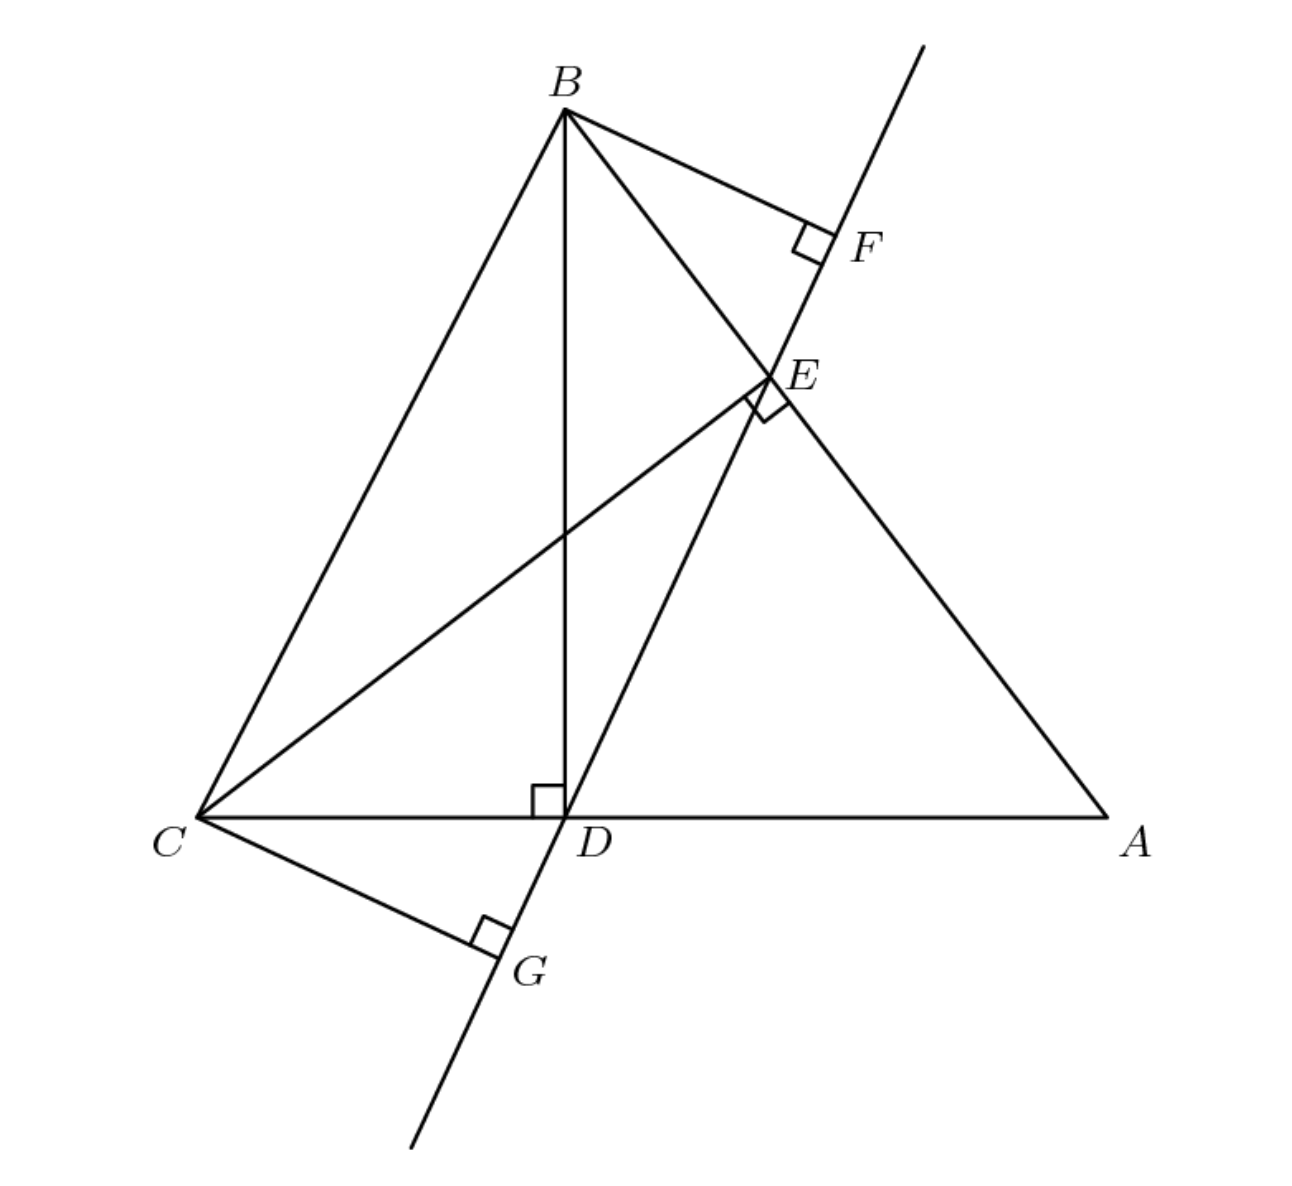
\includegraphics[scale=0.4]{graphics/p2-1.png}
\end{center}
We present two proofs for the problem, though there are many.  The first uses basic facts about cyclic quadrilaterals and similar triangles.
\begin{proof}
Note that $BEDC$ is a cyclic quadrilateral.  Note that $\angle BCD = \angle BEF = 180 - \angle BED$.    Hence, $\triangle BEF \sim \triangle BCD$.  Similarly, $\triangle CGD \sim \triangle CEB$. Therefore,
$$\frac{EF}{CD} = \frac{BE}{BC} = \frac{DG}{CD},$$
so it follows that $EF = DG$.
\end{proof}
The second proof uses properties of projections.
\begin{proof}
The midpoint of $BC$ is the circumcenter of circle $BCDE$, so it projects to the midpoint of $DE$. On the other hand, the midpoint of $BC$ projects to the midpoint of $FG$, since $BFGC$ is a trapezoid. It follows that $DE$ and $GF$ have the same midpoint, so $DG=EF$.
\end{proof}
\subsection{Russia}
\begin{Prob}[Russia] Points $E$ and $F$ are on side $BC$ of a convex quadrilateral $ABCD$ with $BE<BF$.  Given that $\angle BAE = \angle CDF$ and $\angle EAF = \angle FDE$, prove that $\angle FAC = \angle EDB$.
\end{Prob}
\begin{center}
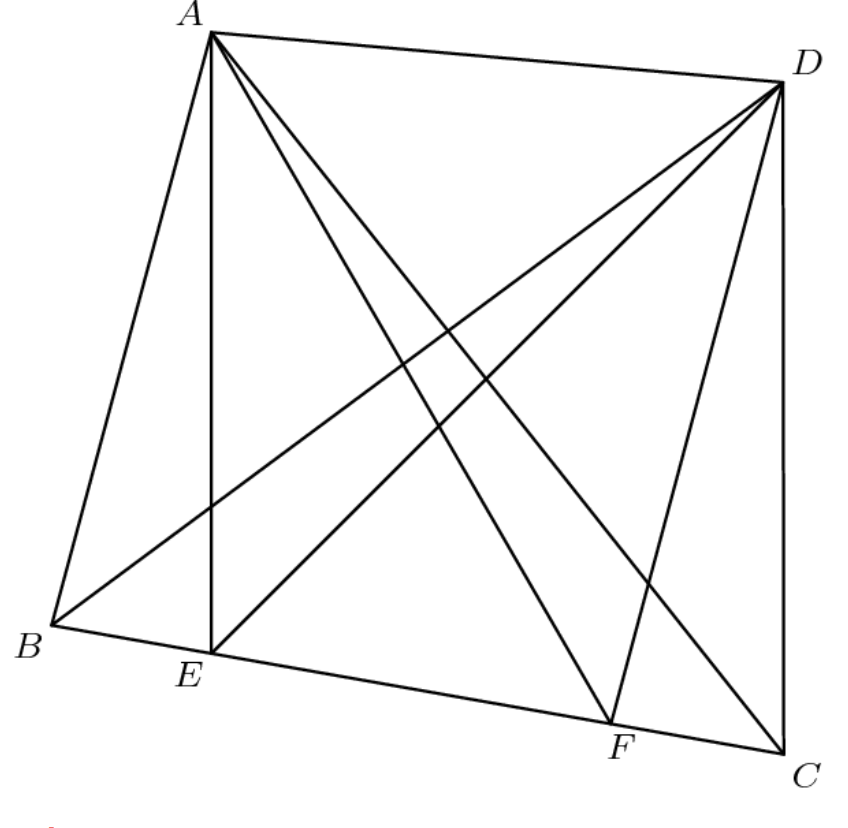
\includegraphics[scale=0.4]{graphics/p2-2.png}
\end{center}
\begin{proof}
Note that $\angle EAF = \angle FDE$ implies that $AEFD$ is cyclic.  It suffices to show that $ABCD$ is cyclic.  Note that $\angle ADC = \angle ADF + \angle FDC$, so we have 
$$\angle ABC + \angle ADC = \angle ABC + \angle ADF + \angle FDC.$$
Then, $\angle ABC = \angle AEF - \angle BAE$, so it follows that 
\begin{align*}
\angle ABC + \angle ADC &= \angle ABC + \angle ADF + \angle FDC \\
&= \angle AEF - \angle BAE + \angle ADF + \angle FDC \\
&= \angle AEF + \angle ADF \\
&= 180,
\end{align*}
which shows that $ABCD$ is cyclic, as desired.
\end{proof}
\subsection{Bulgaria}
\begin{Prob}[Bulgaria] A convex quadrilateral $ABCD$ is given for which $\angle ABC + \angle BCD < 180$.  $AB$ and $CD$ extended meet at $E$.  Prove that $\angle ABC = \angle ADC$ if and only if $AC^2= CD \cdot CE - AB \cdot AE$.
\end{Prob} 
\begin{remark} After drawing the diagram for the problem, one should check that it corresponds to the solution in the problem.  One can enter a trap proceeding without checking for this problem specifically.
\end{remark}
\begin{center}
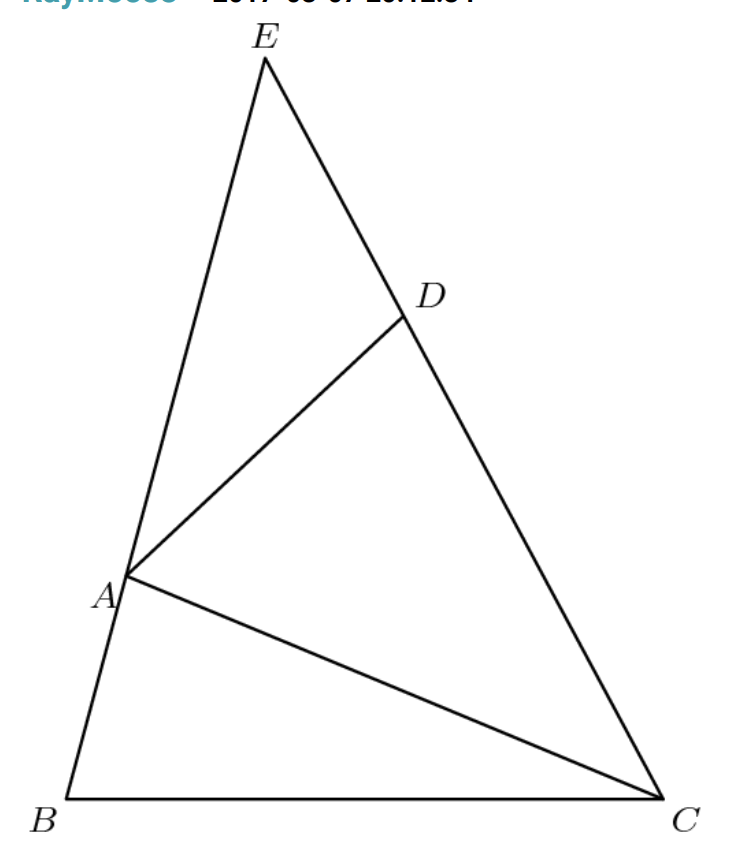
\includegraphics[scale=0.4]{graphics/p2-3.png}
\end{center}
\begin{proof}
Let $\omega_1$ be the circumcircle of $ADE$ and $\omega_2$ be the circumcircle of $EBC$.  Note that $\text{Pow}_{\omega_1}(C) = CD \cdot CE$ and $\text{Pow}_{\omega_2}(A) = AB \cdot AE$.  Extend $CA$ to $\omega_2$ and label the intersection $F$.  
\begin{center}
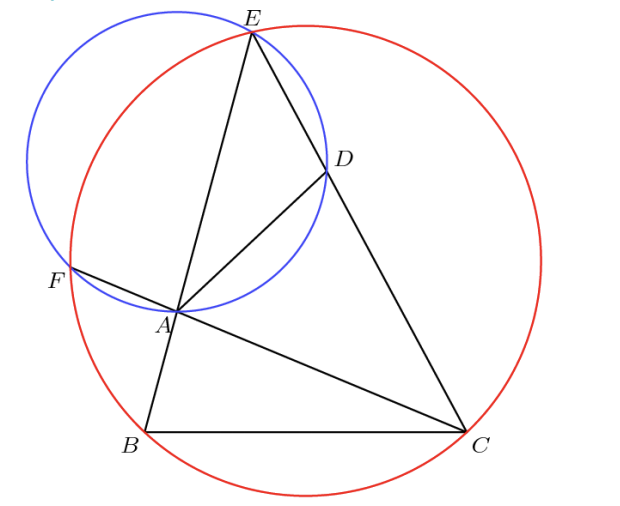
\includegraphics[scale=0.7]{graphics/p2-4.png}
\end{center}
Assuming that $AC^2 = CD \cdot CE - AB \cdot AE = CA \cdot CF - AB \cdot AE$, it follows that 
$$AC(CF - AC) = AC \cdot AF = AB \cdot AE,$$
so from the converse of the Power of a Point, it follows that $F \in \omega_2$.

Finally,
$$\angle ABC = \angle AFE = 180 - \angle ADE = \angle ADC.$$

We can go back and show that each of the steps are reversible, but this is left as an exercise.
\end{proof}


\subsection{Iran}
\textbf{Warning}: This is a very difficult problem.
\begin{Prob}[Iran] Point $K$ is outside circle $C$ and points $L$ and $N$ are on $C$ such that $KL$ and $KN$ are tangent to $C$.  Let $M$ be on ray $KN$ beyond $N$, and let $P$ be the second intersection of the circumcircle of $KLM$ and $C$.  Let $Q$ be the foot of the perpendicular from $N$ to $ML$.  Prove that $\angle MPQ = 2\angle KML$.
\end{Prob}
\begin{center}
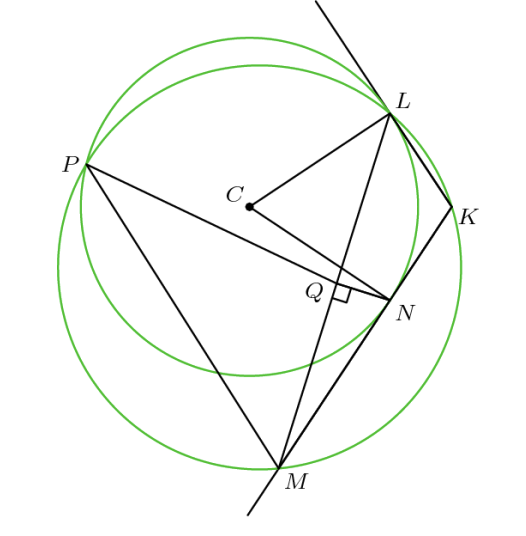
\includegraphics[scale=0.7]{graphics/p2-5.png}
\end{center}
\begin{proof}
Let $S$ be the intersection of $QM$ and circle $C$.  We show that $PS$ bisects $P$.  Let $T$ be the intersection of $PM$ and $(PNL)$.   
\begin{center}
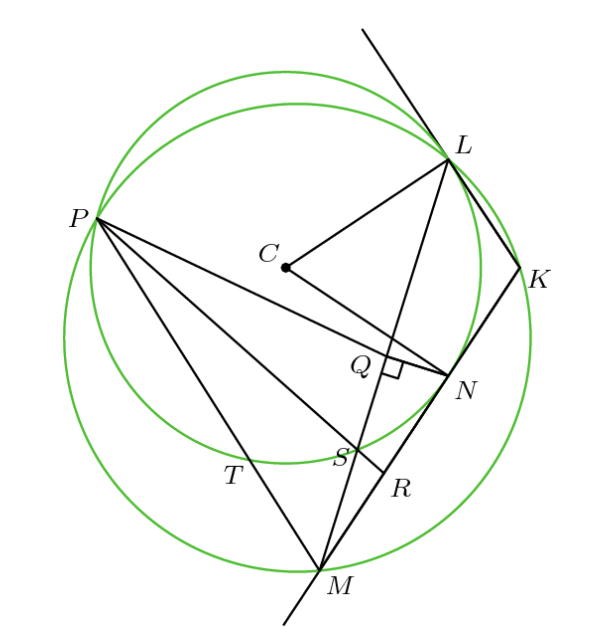
\includegraphics[scale=0.7]{graphics/p2-6.png}
\end{center}

We would like to show that $\angle QPS = \angle MPS = \angle KML$.  First, note that $\angle KML = \angle KPL$ since they are inscribed in the same arc $LK$ of $(KLPM)$.   If we can show $\angle MPK = \angle SPL$, this shows that $\angle KPL = \angle MPS$ since they share a common angle $\angle SPK$, and hence $\angle KML = \angle MPS$.

Firstly, $\angle MLK = \angle MPL$ from cyclic quadrilateral $MKLP$.  Then, $\angle MLK = \angle SLK = \angle SPL$ since they are inscribed in arc $LS$ of circle $C$.  Thus, $\angle KML = \angle MPS$.
\begin{center}
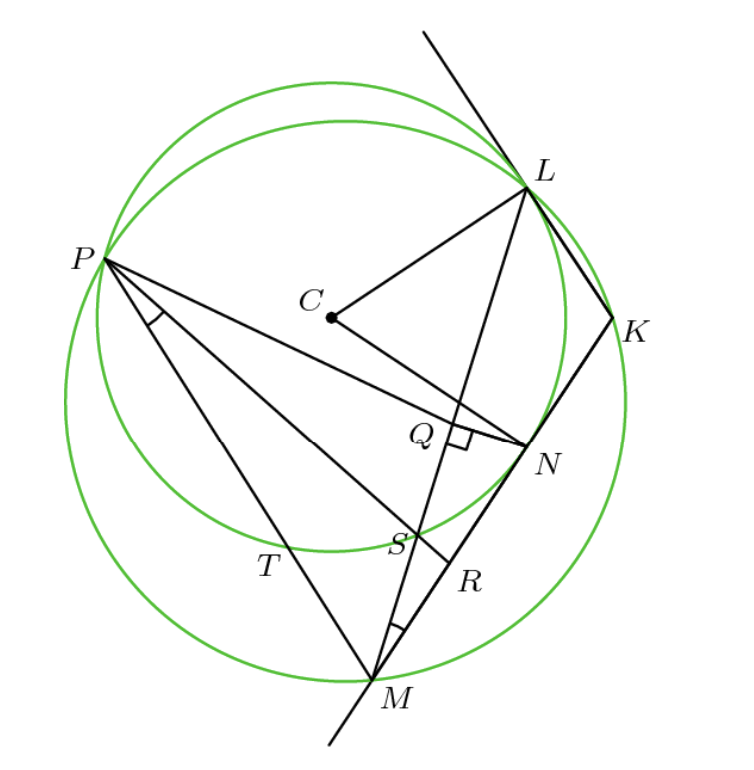
\includegraphics[scale=0.6]{graphics/p2-7.png}
\end{center}
It suffices to show that either $\angle KML = \angle QPS$ or $\angle MPS = \angle QPS$.  To show the first, we can show that $PQRM$ is cyclic.  A good candidate to show this is to show that $\angle RQM = \angle RPM$, since we already know that $\angle RPM = \angle RMS$.    To show $\angle RQM = \angle RMS$, it suffices to show that $RQM$ is isosceles, or $RQ = RM$.  

Note that $\triangle PRM \sim \triangle MRS$ since they share $\angle SRM$ and $\angle SMR = \angle MPR$.  From this, we find that 
$$\frac{PR}{MR} = \frac{RM}{RS} = \frac{MP}{SM} \Longrightarrow MR^2 = RP \cdot RS.$$
Then,
$$\text{Pow}_C(R) = RN^2 = RS \cdot RP = RM^2,$$
so it follows that $RM = RN$ so $R$ is the center of $(MQN)$ and it follows that $RQ = RM$, as desired.  Therefore,
$$\angle QPM = \angle QPR + \angle RPM = \angle KML + \angle KML = 2\angle KML,$$
as desired.
\end{proof}
\end{document}
